En esta sección el objetivo será comparar todos los algoritmos diseñados e implementados en este trabajo.

A continuación incluiremos dos gráficos. Uno para poder observar como se comportan tanto nuestros algoritmos ante la familia de grafos \emph{3-caminos} y otro ante la familia \emph{3-caminos con puentes}.

\begin{figure}[H]
    \begin{minipage}{0.5\linewidth}
      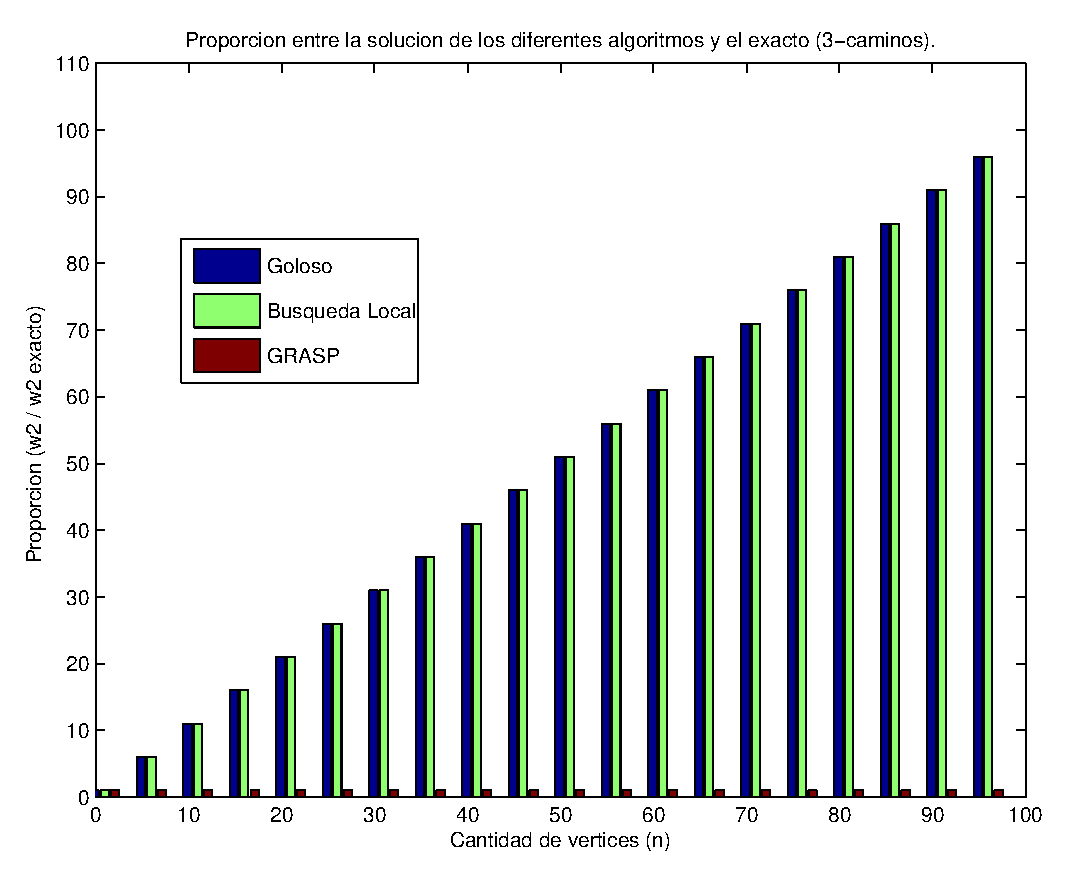
\includegraphics[width=\linewidth]{graficos/todos_proporcion_3caminos.eps}
      \caption{Comportamiento ante familia \emph{3-caminos}}\label{fig:comportamiento-familia-rompe}
    \end{minipage}
    \hfill
    \begin{minipage}{0.5\linewidth}
      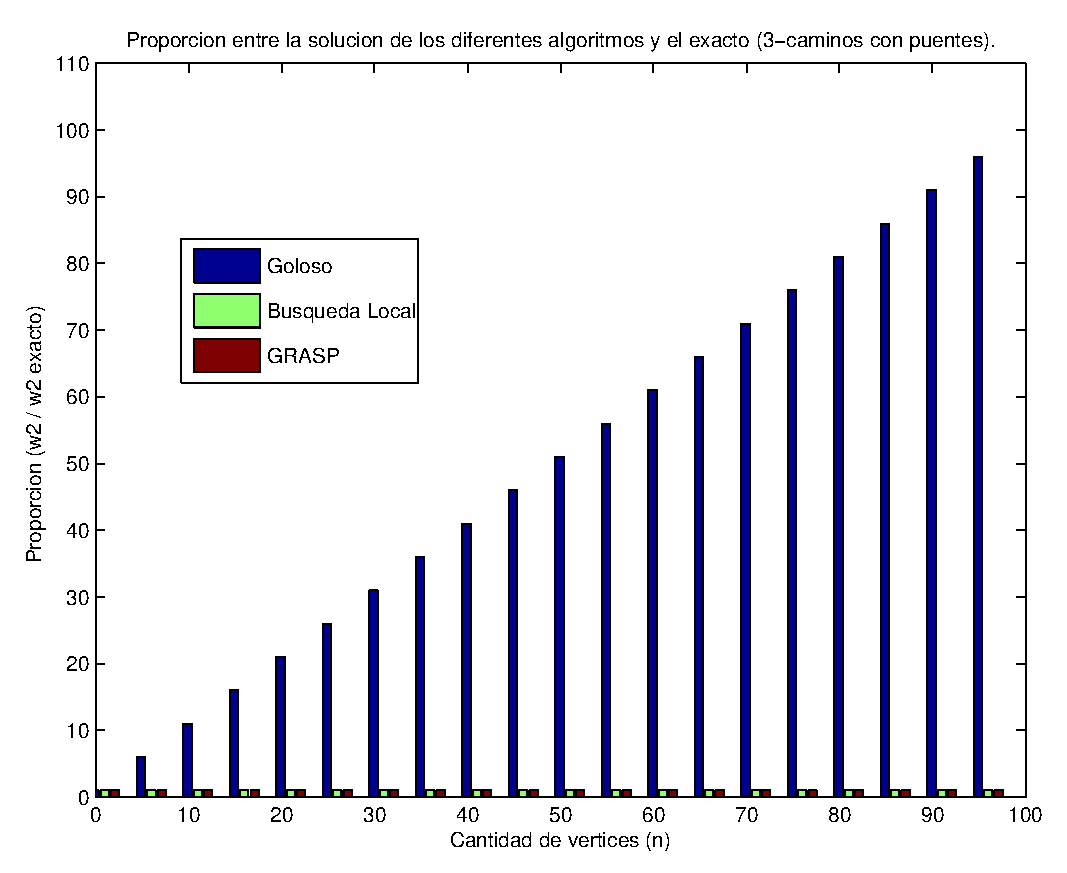
\includegraphics[width=\linewidth]{graficos/todos_proporcion_puentes.eps}
      \caption{Idem familia \emph{3-caminos con puentes}}\label{fig:comportamiento-familia-puente}
    \end{minipage}    
\end{figure}

En estos gráficos mostramos el comportamiento de tanto de los siguientes algoritmos para dos famlias de grafos. Los algoritmos medidos son los siguientes (todos en proporción al algoritmo exacto):


\begin{itemize}
 \item Algoritmo Goloso implementado en el trabajo
 \item Algoritmo de búsqueda local con algoritmo goloso como semilla
\end{itemize}


En el gráfico de la Figura \ref{fig:comportamiento-familia-rompe} podemos ver que para los grafos de la familia \emph{3-caminos} nuestro algoritmo GRASP